\documentclass[twocolumn]{article}
\usepackage{amsmath}
\usepackage{amsfonts}
\usepackage{amsthm}
\usepackage{graphicx}
\usepackage{thmtools}
\usepackage{hyperref}
\input{sym}

\title{Midterm 1  Review}
\author{Vikas  Dhiman}
\newtheorem{thm}{Theorem}
\newtheorem{defn}{Definition}
\newtheorem{exmpl}{Example}

\DeclareMathOperator{\atantwo}{atan2}

\begin{document}
\maketitle

\tableofcontents
\section{Linear algebra   review}
\begin{defn}[Matrix] A  real  matrix  $A$ with $n$ rows  and  $m$  columns is defined as a  set  of real numbers  $\{a_{11}, a_{12},
\dots,     a_{nm}\}$, arranged in
an 2D grid with $n$  rows  and $m$  columns :
\begin{align}
  A  =  \begin{bmatrix}
    a_{11}  &  a_{12} &   \dots &  a_{1m} \\
    a_{21}  &  a_{22} &   \dots &  a_{2m} \\
    \vdots  & \vdots &   \ddots  &  \vdots   \\
    a_{n1}  &  a_{n2} &   \dots &  a_{nm} \\
    \end{bmatrix}
\end{align}
\end{defn}

The set of all possible real  matrices with  $n$ rows   and   $m$  columns  is
denoted  as $\bbR^{n \times   m}$, where  $\bbR$ denotes  the set  of all real numbers.

Any matrix $A$ with with  $n$  rows  and  $m$  columns  is   said  to lie  in
the  set  of $\bbR^{n \times   m}$. $A \in \bbR^{n \times m}$  is  read aloud
as ``$A$  lies  in   the set of all $n$ cross $m$  real matrices''.

\begin{defn}[Vector  or Column vector]
  A column vector or a vector $\bfx$ is a matrix  with only one column.
  \begin{align}
    \bfx  =  \begin{bmatrix}
      x_{1} \\
      x_{2} \\
      \vdots   \\
      x_{n} \\
    \end{bmatrix}
  \end{align}
\end{defn}

The set of all possible real  vectors with  $n$ rows   is
denoted  as $\bbR^{n \times   1}$ or more simply $\bbR^{n}$.

A vector is denoted by bold-font small letter, for example, $\bfx, \bfy, \bfz$.
A  matrix is denoted by capital letters, $A, B, M, P, K$.

A matrix $A  \in \bbR^{n \times  m}$ is often denoted a set $m$ column vectors
of dimension $n   \times  1$,
%
\begin{align}
  A  &=  \begin{bmatrix}
    \bfa_1 &  \bfa_2 &  \dots & \bfa_m
  \end{bmatrix},
 \notag\\
 \text{where   }   \bfa_i &= \begin{bmatrix}
 a_{i1} \\  a_{i2} \\ \vdots \\ a_{in}
 \end{bmatrix}, \qquad  \text{ for all } i  \in \{1, \dots, m\}.
\end{align}
%

A block matrix  is a matrix denoted in terms  of  other matrices,
%
\begin{align}
  A &= \left[\begin{array}{ccc|ccc}
        b_{11} & \dots  &   b_{1q}  &   c_{11}  &   \dots   & c_{1r} \\
        \vdots  &  \ddots   & \vdots &  \vdots  &  \ddots  &  \vdots  \\
        b_{p1} & \dots  &   b_{pq}  &   c_{1s}  &   \dots   & c_{sr} \\
        \cline{1-6}  \\
        e_{11} & \dots  &   e_{1v}  &   d_{11}  &   \dots   & d_{1x} \\
        \vdots  &  \ddots   & \vdots &  \vdots  &  \ddots  &  \vdots  \\
        e_{u1} & \dots  &   e_{uv}  &   d_{1w}  &   \dots   & d_{wx} \\
            \end{array}\right]
  \\
    &= \begin{bmatrix}
        B  &   C \\
        E & D
        \end{bmatrix}, \text{  where  }  B, C, E, D \text{ are matrices.}
\end{align}
%

\begin{defn}[Square matrix]
  A matrix is said to be square if its number of columns is same as the number
  of rows. That is matrix   $A \in \bbR^{n \times m}$ is said to be square
  matrix if $m = n$.
\end{defn}

\begin{defn}[Diagonal of a square matrix]
  Let $A$ be a square matrix $A \in \bbR^{n \times n}$  with   entries:
  \begin{align}
    A  =  \begin{bmatrix}
      a_{11}  &  a_{12} &   \dots &  a_{1n} \\
      a_{21}  &  a_{22} &   \dots &  a_{2n} \\
      \vdots  & \vdots &   \ddots  &  \vdots   \\
      a_{n1}  &  a_{n2} &   \dots &  a_{nn} \\
    \end{bmatrix}
  \end{align}
  The diagonal of a square matrix  $A$ is defined  to be the vector
  \[  \text{diag}(A)= \begin{bmatrix} a_{11} \\   a_{22} \\ \vdots  \\ a_{nn} \end{bmatrix}\]
\end{defn}

\begin{defn}[Identity matrix]
  An identity matrix $I$ of size $n$ is  a square matrix with all its diagonal
  entries as 1 and non-diagonal entries as 0.
  \begin{align}
    I  =  \begin{bmatrix}
      1 & 0 & \dots & 0   \\
      0 & 1 & \dots & 0   \\
      \vdots   & \vdots &  \ddots  & \vdots \\
      0 & 0 & \dots & 1   \\
      \end{bmatrix}
    \end{align}
\end{defn}


\subsection{Matrix operations}
\subsubsection{Transpose}
\begin{defn}[Transpose]
  The matrix transpose $A^\top$ of a matrix $A$ is defined as a matrix where
  rows of matrix $A$ are the columns  of $A^\top$ and vice-versa.
  \begin{align}
    A^\top  =  \begin{bmatrix}
      a_{11}  &  a_{21} &   \dots &  a_{1n} \\
      a_{12}  &  a_{22} &   \dots &  a_{2n} \\
      \vdots  & \vdots &   \ddots  &  \vdots   \\
      a_{1m}  &  a_{2m} &   \dots &  a_{nm} \\
    \end{bmatrix}
  \end{align}
\end{defn}

In  the matrix as set of  $m$ column  vectors notation, the transpose is written as $m$
row  vectors $\bfa_i^\top$,
%
\begin{align}
  A^\top  &=  \begin{bmatrix}
    \bfa_1^\top \\ \bfa_2^\top \\ \vdots \\  \bfa_m^\top
  \end{bmatrix},
  \quad
  \bfa_i^\top = \begin{bmatrix}
    a_{i1}  & a_{i2}  &   \dots &  a_{in}
  \end{bmatrix},
                                  \notag \\
  &\qquad \text{for all } i \in \{1, \dots, n\}.
\end{align}
%

\begin{enumerate}
\item  If $A$ has $n$rows and  $m$  columns, then  $A^\top$  has $m$ rows and
  $n$  columns. If  $A \in \bbR^{n \times  m}$, then  $A^\top \in \bbR^{m
    \times n}$.
  \item  The transpose  of  a transpose is matrix itself. $(A^\top)^\top = A$.
  \item  The transpose of a block matrix is  block-wise  transpose  of  each
    matrix,
    \[
    \begin{bmatrix}
      B  &   C \\
      E & D
    \end{bmatrix}^\top
    = 
    \begin{bmatrix}
      B^\top  & E^\top \\
      C^\top & D^\top
    \end{bmatrix}
    \]
    
\end{enumerate}


\begin{defn}[Row vector]
  A row vector is $Y$ is matrix  with only one row
  \begin{align}
    Y  =  \begin{bmatrix}
      y_{1} &
      y_{2} &
      \dots  &
      y_{n}
    \end{bmatrix}
  \end{align}
\end{defn}
It is common  to denote row vectors as tranpose  of  a  column vector. For
example, the  matrix  $Y$ shown above is typically represented  $\bfy^\top$, where
$\bfy$  is a column vector.
%
  \begin{align}
    Y  &=  \bfy^\top & \text{ where } \bfy = \begin{bmatrix}
      y_{1} \\
      y_{2} \\
      \vdots  \\
      y_{n}
    \end{bmatrix}
  \end{align}

\subsubsection{Vector dot product}
Before we define  general matrix multiplication, it  is easier to define matrix
multiplication   between a row vector and a column vector $\bfx^\top  \in
\bbR^{1 \times  n}$ and $\bfy\in\bbR^{n \times 1}$
%
\begin{align}
  \bfx^\top \bfy  &= x_1y_1 + x_2 y_2 + \dots  + x_n y_n = \sum_{i=1}^n  x_iy_i
\\
\text{where }  \bfx^\top &=  \begin{bmatrix} x_1 &  \dots  &  x_n \end{bmatrix}
\notag \\
  \text{  and  }\bfy &=  \begin{bmatrix} y_1 \\  \vdots  \\  y_n \end{bmatrix}.
  \notag
\end{align}
%
Note that $\bfx^\top \bfy$   is same as the vector  dot product  or the vector
inner-product,
%
\begin{align}
  \bfx^\top \bfy = \bfx \cdot \bfy  =  \|\bfx\|\|\bfy\|cos(\theta) = \bfy^\top \bfx,
\end{align}
  %
where  $\theta$  is the angle between   vectors $\bfx$ and $\bfy$ and  the
vector norm  or euclidean norm $\|.\|$ is defined as
%
\begin{align}
  \|\bfx\| =  \sqrt{x_1^2 + x_2^2  +   \dots +  x_n^2} = \sqrt{\bfx^\top\bfx}
\end{align}
%

\begin{defn}[Unit  vector]
  A unit vector, typically denoted  with a hat, $\hat{\bfx}$ is a vector with
  euclidean norm as 1. That is  $\|\hat{\bfx}\| = 1$ or equivalently
  $\bfx^\top\bfx =  1$.
\end{defn}

\begin{defn}[Orthogonal vectors]
  Two vectors, $\bfx \in  \bbR^n$  and $\bfy \in \bbR^n$ are said to be
  orthogonal if and only if their dot product is zero $\bfx^\top \bfy =  0$.
\end{defn}

\begin{defn}[Orthonormal vectors]
  A set of vectors, $\bfx_1, \bfx_2, \dots, \bfx_n \in  \bbR^n$  are said to be
  orthonormal if and only if they are all  unit vectors $\bfx_i^\top\bfx_i  = 1$
  and they are  pair-wise orthogonal, $\bfx_i^\top  \bfx_j =  0$ for all $i \ne j$. 
\end{defn}

\subsubsection{Matrix multiplication}
The matrix multiplication between  matrix  $A \in \bbR^{n  \times m}$   and
matrix $B  \in \bbR^{m \times p}$ (note that $A$ has $m$ columns while B has $m$
rows;  the only case when matrix multiplication  is defined) is easier 
defined if matrix $A$  is written in terms  of row vectors while  matrix  $B$ is
written  in  terms  of column vectors. Let  the  matrix $A$  is written in terms
of row   vectors $\bfa_i^\top   \in \bbR^{1 \times m}$ and the matrix $B$ is written in terms of column
vectors $\bfb_i \in \bbR^{m \times  1}$. Then the matrix multiplication $AB \in
\bbR^{n \times  p}$ is defined as the matrix,
%
\begin{align}
  AB &= \begin{bmatrix}
    \bfa_1^\top
    \\
    \bfa_2^\top
    \\
    \vdots
    \\
    \bfa_n^\top
    \end{bmatrix}
  \begin{bmatrix}
    \bfb_1
    &
    \bfb_2
    &
    \dots
    &
    \bfb_p
  \end{bmatrix}
      \\
  &= \begin{bmatrix}
    \bfa_1^\top\bfb_1 & \bfa_1^\top\bfb_2 &  \dots & \bfa_n^\top \bfb_p
    \\
    \bfa_2^\top\bfb_1 & \bfa_2^\top\bfb_2 &  \dots & \bfa_n^\top \bfb_p
    \\
    \vdots &  \vdots  &  \ddots  &   \vdots
    \\
    \bfa_n^\top\bfb_1 & \bfa_n^\top\bfb_2 &  \dots & \bfa_n^\top \bfb_p
    \end{bmatrix}
\end{align}

\paragraph{Block matrix  multiplication}
Block matrix multiplication works in a similar way  as scalar multiplication as
long as sub-matrix multiplication is properly defined,
%
\begin{align}
  \begin{bmatrix}  A & B \\  C &  D \end{bmatrix}
  \begin{bmatrix}  P & Q \\  R &  S \end{bmatrix}
 =
   \begin{bmatrix}  AP+BR & AQ+BS \\  CP+DR &  CQ+DS \end{bmatrix}
  \end{align}
  %

\begin{defn}[Orthogonal matrices]
  A square matrix $A$ is said to be orthogonal if and only if $A^\top A = I$
\end{defn}

\subsubsection{Transpose of matrix multiplication}
\[
  (AB)^\top = B^\top A^\top
  \]


\section{Trignometry review}

\includegraphics[width=\linewidth]{media/trig.pdf}

\section{Triangle law of vector addition}

\includegraphics[width=\linewidth]{media/triangle-law.png}

\section{2D  Rotation matrix}
\begin{defn}[2D  Cartesian Coordinate frame]
 A 2D cartesian coordinate  frame  is defined as a set of mutually orthogonal unit
 vectors  $\hat{\bfx} \in  \bbR^2$  and
 $\hat{\bfy}\in  \bbR^2 $ called the basis vectors $B = [\hat{\bfx}, \hat{\bfy}]$
 along  with  an origin  $\bfo\in  \bbR^2$. Thus the tuple  $(B, \bfo)$ form a
 coordinate frame. A  coordinate  frame is denoted  by curly braces around it,
 for  example, $\{C\}$ or $\{W\}$.
\end{defn}

\begin{exmpl}[2D Coordinate frame]
  The figure~\ref{fig:rot-2D} contains two coordinate frames the one  shown  in
  red and   the one   shown in green. Both have  the  same origin, but
  different  basis vectors. The $\{W\}$ coordinate frame shown in green has
  basis vectors $B_w = [\hat{\bfx}_w, \hat{\bfy}_w]$. The same notation is used
  for the $\{C\}$ coordinate frame $B_c  =  [ \hat{\bfx}_c, \hat{\bfy}_c]$.
  Note that the basis vectors of $\{C\}$  coordinate frame  can be
  expressed  in  terms of $\{W\}$  coordinate frame by triangle  law of vector addition,
  \begin{equation}
  \begin{aligned}
    \hat{\bfx}_c &= |\overrightarrow{OA}|\hat{\bfx}_w + |\overrightarrow{AB}|\hat{\bfy}_w
    \\
    \hat{\bfy}_c &= -|\overrightarrow{PQ}|\hat{\bfx}_w + |\overrightarrow{OP}|\hat{\bfy}_w
  \end{aligned}
  \label{eq:c-as-w}
  \end{equation}

  In the  triangle $\Delta OAB$ (Fig~\ref{fig:rot-2D}),
  \begin{align}
    \cos(\theta) &= \frac{|\overrightarrow{OA}|}{|\overrightarrow{OB}|}
                   = \frac{|\overrightarrow{OA}|}{\|\hat{\bfx}_c\|} = |\overrightarrow{OA}| \\
    \sin(\theta) &= \frac{|\overrightarrow{AB}|}{|\overrightarrow{OB}|}
                   = \frac{|\overrightarrow{AB}|}{\|\hat{\bfx}_c\|} =|\overrightarrow{AB}|
  \end{align}
  Similarly in  the  right  triangle $\Delta OPQ$ (Fig~\ref{fig:rot-2D}),
  \begin{align}
    \cos(\theta) &= \frac{|\overrightarrow{OP}|}{|\overrightarrow{OQ}|}
                   = \frac{|\overrightarrow{OP}|}{\|\hat{\bfy}_c\|} = |\overrightarrow{OP}| \\
    \sin(\theta) &= \frac{|\overrightarrow{PQ}|}{|\overrightarrow{OQ}|}
                   = \frac{|\overrightarrow{PQ}|}{\|\hat{\bfy}_c\|} =|\overrightarrow{PQ}|
  \end{align}
  Putting  these values back  in  
  \eqref{eq:c-as-w}, we get,
  \begin{equation}
    \begin{aligned}
      \hat{\bfx}_c &= cos(\theta)\hat{\bfx}_w + sin(\theta)\hat{\bfy}_w
      \\
      \hat{\bfy}_c &= -sin(\theta)\hat{\bfx}_w + cos(\theta)\hat{\bfy}_w
    \end{aligned}
  \end{equation}
  These equations can be written in matrix notation as,
  \begin{equation}
    \begin{aligned}
      \hat{\bfx}_c &= \begin{bmatrix}\hat{\bfx}_w & \hat{\bfy}_w\end{bmatrix}
      \begin{bmatrix}cos(\theta)  \\  sin(\theta) \end{bmatrix} = B_w\begin{bmatrix}cos(\theta)  \\  sin(\theta) \end{bmatrix}
      \\
      \hat{\bfy}_c &= \begin{bmatrix}\hat{\bfx}_w & \hat{\bfy}_w\end{bmatrix}
      \begin{bmatrix}
        -sin(\theta)  \\ cos(\theta)  \end{bmatrix}= B_w\begin{bmatrix}
        -sin(\theta)  \\ cos(\theta)  \end{bmatrix}
    \end{aligned}
  \end{equation}
  The full  basis matrix of coordinate frame $\{C\}$ can be   written as
    \begin{equation}\begin{aligned}
    B_c &= \begin{bmatrix} \hat{\bfx}_c & \hat{\bfy}_c  \end{bmatrix}
    \\
        &= \begin{bmatrix}
          B_w\begin{bmatrix}cos(\theta)  \\  sin(\theta) \end{bmatrix} 
          & B_w\begin{bmatrix}-sin(\theta)  \\  cos(\theta) \end{bmatrix} 
        \end{bmatrix}
    \\
    &= B_w\begin{bmatrix} cos(\theta) &  -sin(\theta)  \\  sin(\theta) &  cos(\theta)\end{bmatrix} 
  \end{aligned}
  \label{eq:basis-c-in-basic-w}
\end{equation}
\end{exmpl}

\begin{defn}[2D Coordinates of a  point]
  The coordinate of a point $\bfp$ in a given coordinate frame $\{W\}$ with
  basis vectors $B_w =  [\hat{\bfx}_w, \hat{\bfy}_w]$ and origin $\bfo_w
  = \begin{bmatrix} o_x \\ o_y \end{bmatrix}$ is
  defined as the vector $\bfp_w = \begin{bmatrix} p_{wx}  \\
    p_{wy}  \end{bmatrix}$  such that,
  \begin{align}
    \bfp &= (p_{wx} + o_x)\hat{\bfx}_w + (p_{wy} + o_y)\hat{\bfy}_w\notag\\
    &=  \begin{bmatrix} \hat{\bfx}_w & \hat{\bfy}_w \end{bmatrix} \left(\begin{bmatrix} p_{wx} \\  p_{wy} \end{bmatrix} +  \begin{bmatrix}o_x \\ o_y \end{bmatrix}  \right)
    \notag\\
    &=  B_w(\bfp_w +   \bfo_w)
  \end{align}
\end{defn}

\begin{exmpl}[Fig~\ref{fig:rot-2D}]
  The point $\bfp$ can be represented in coordinate frames $\{W\}$ and  $\{C\}$.
  Let the projection on the basis $B_c = [\hat{\bfx}_c, \hat{\bfy}_c]$ be
  $\bfp_c$, while that on $B_w  = [\hat{\bfx}_w, \hat{\bfy}_w]$ be $\bfp_w$.
  Since both the coordinate  frames have same origin, we  assume $\bfo_w =
  \bfo_c = \begin{bmatrix}  0  \\  0 \end{bmatrix}$. We have
  %
  \begin{align}
    \bfp &=  B_w\bfp_w =  B_c\bfp_c
           \label{eq:pt-as-basis}
  \end{align}
  %
\end{exmpl}

\begin{thm}[2D  Rotation matrix]
  In a coordinate transformation  as  given in Fig~\ref{fig:rot-2D}, the
  coordinates in  frame $\{C\}$, $\bfp_c$ can be
  converted   into coordinates in frame $\{W\}$, $\bfp_w$ with the same  origin
  by using a  rotation matrix  ${}^WR_C(\theta)$,
  \begin{align}
    \bfp_w  &=  {}^WR_C(\theta)\bfp_c
              \notag\\
    \text{where  }  {}^WR_C(\theta) &= \begin{bmatrix}
      cos(\theta) &  -sin(\theta) \\
      sin(\theta) &  cos(\theta)
      \end{bmatrix}
    \end{align}
\end{thm}
\begin{proof}
  First note  that the basis matrix of any coordinate frame $\{W\}$ is
  orthogonal,
  \begin{align}
    B_w^\top B_w &= \begin{bmatrix}  \hat{\bfx} &  \hat{\bfy} \end{bmatrix}^\top
         \begin{bmatrix}  \hat{\bfx} &  \hat{\bfy} \end{bmatrix}
    \notag\\
    &=
    \begin{bmatrix}  \hat{\bfx}^\top \\  \hat{\bfy}^\top \end{bmatrix}
                                  \begin{bmatrix}  \hat{\bfx} &  \hat{\bfy} \end{bmatrix}
    \notag\\
    &=   \begin{bmatrix}  \hat{\bfx}^\top\hat{\bfx}  &   \hat{\bfx}^\top\hat{\bfy}
      \\  \hat{\bfy}^\top\hat{\bfx}  &  \hat{\bfy}^\top\hat{\bfy} \end{bmatrix}
    \notag\\
                 &=  \begin{bmatrix}
                   1 &  0  \\   0   &  1
                 \end{bmatrix} = I
  \end{align}

  Left-multiply $B_w^\top$ to both sides of \eqref{eq:pt-as-basis}
  \begin{align}
    B_w^\top  B_w \bfp_w = B_w^\top   B_c  \bfp_c
    \end{align}
    Cancel out $B_w^\top \bfo$ on both sides.  Replace $B_w^\top  B_w = I$.
    \begin{align}
      I \bfp_w = B_w^\top   B_c  \bfp_c
      \text{ or } \bfp_w = B_w^\top   B_c  \bfp_c
    \end{align}
    Substitute value  of $B_c$  from 
    \eqref{eq:basis-c-in-basic-w}, to get
    \begin{align}
      \bfp_w = B_w^\top   \left( B_w  \begin{bmatrix} \cos(\theta) &  -\sin(\theta) \\
        \sin(\theta) &   \cos(\theta) \end{bmatrix}   \right)\bfp_c.
    \end{align}
    Again  use $B_w^\top  B_w = I$ to get,

    \begin{align}
      \bfp_w = \begin{bmatrix} \cos(\theta) &  -\sin(\theta) \\
          \sin(\theta) &   \cos(\theta) \end{bmatrix} \bfp_c.
    \end{align}

    Defining ${}^WR_C(\theta) = \begin{bmatrix} \cos(\theta) &  -\sin(\theta) \\
      \sin(\theta) &   \cos(\theta) \end{bmatrix}$, we get the desired result.

    \end{proof}

\begin{figure}
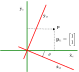
\includegraphics[width=\linewidth]{media/rot-2D.pdf}
\caption{The coordinate  frame $\{C\}$  is rotated around origin by an $\theta$
  from coordinate  frame $\{W\}$.}
\label{fig:rot-2D}
\end{figure}

\begin{thm}[Orthogonality of 2D Rotation matrices]
  All 2D rotation matrices  are orthogonal $R^\top R = I$ have determinant as one
  $\det(R) =  1$. If any square matrix $A \in \bbR^{2\times  2}$ is orthogonal $A^\top A = I$  and has
  determinant 1, $\det(A) = 1$, then  it is a valid rotation matrix.
\end{thm}
\begin{proof}
  \begin{align}
    R^\top R
    &= \begin{bmatrix}
      \cos(\theta)  &  -\sin(\theta)
      \\
      \sin(\theta) &   \cos(\theta)
    \end{bmatrix}^\top \begin{bmatrix}
      \cos(\theta)  &  -\sin(\theta)
      \\
      \sin(\theta) &   \cos(\theta)
    \end{bmatrix}
    \notag\\
    &=\begin{bmatrix}
      \cos(\theta)  &  \sin(\theta)
      \\
      -\sin(\theta) &   \cos(\theta)
    \end{bmatrix} \begin{bmatrix}
      \cos(\theta)  &  -\sin(\theta)
      \\
      \sin(\theta) &   \cos(\theta)
    \end{bmatrix}
  \notag\\
    &=\begin{bmatrix}
      \cos^2(\theta)+\sin^2(\theta)  &  -\cos(\theta)\sin(\theta)+\sin(\theta)\cos(\theta)
      \\
      -\sin(\theta)\cos(\theta)+\cos(\theta)\sin(\theta) &   \sin^2(\theta)+\cos^2(\theta)
    \end{bmatrix}
\notag\\
    &=\begin{bmatrix}
      1  &  0  \\ 0  &   1\end{bmatrix}
    \end{align}
    \begin{align}
      \det(R) &
                =  \det\begin{bmatrix}
        \cos(\theta)  &  -\sin(\theta)
        \\
        \sin(\theta) &   \cos(\theta)
        \end{bmatrix}
                       \notag\\
              &= \cos^2(\theta)+  \sin^2(\theta)  = 1
      \end{align}
  Denote the columns of square matrix $A$ which  is orthogonal with determinant
  1 as $A = [\bfa_1, \bfa_2]$. Since $A$ is orthogonal,  we have
  \begin{align}
    A^\top A
    &= \begin{bmatrix}
      \bfa_1^\top  \\   \bfa_2^\top
    \end{bmatrix}
    \begin{bmatrix}
      \bfa_1  &   \bfa_2
    \end{bmatrix}  = \begin{bmatrix} \bfa_1^\top \bfa_1  & \bfa_1^\top \bfa_2
      \\
      \bfa_2^\top \bfa_1 & \bfa_2^\top \bfa_2\end{bmatrix}
      \notag\\
    &= \begin{bmatrix} 1  &  0   \\  0  &  1 \end{bmatrix}.
  \end{align}
  This   implies that $\bfa_1$  and  $\bfa_2$ are mutually orthogonal unit
  vectors. Let $\bfa_1  = [\cos(\theta), \sin(\theta)]$ because any 2D unit
  vector can  be written in cos,sin form, where $\theta = \atantwo(a_{12}, a_{11})$.
  Next we know  that  $\bfa_1^\top\bfa_2 =  0$ and that $\bfa_2$ is unit  vector.
  For any  unit 2D vector   $[u, v]^\top$, there are only two unit vectors
  perpendicular to it $[-v, u]^\top$ and $[v, -u]^\top$.
  Then we have only two
  options for $\bfa_2$  are  either $[-\sin(\theta), \cos(\theta)]$ or
  $[\sin(\theta), -\cos(\theta)]$.  But we also  know that the determinant of
  $A$ is  1. The second option   for $\bfa_2$ leads to determinant of -1.
  \begin{align}
    \det\begin{bmatrix}
      \bfa_1  &  \bfa_2
      \end{bmatrix}
    &=  
      \det\begin{bmatrix}
        \cos(\theta)  &  \sin(\theta)\\
        \sin(\theta) &  -\cos(\theta)
      \end{bmatrix} = -1
    \end{align}
    Hence, we have
    \[
      A = \begin{bmatrix}
        \bfa_1  &  \bfa_2
      \end{bmatrix}
      =  
      \begin{bmatrix}
        \cos(\theta)  &  -\sin(\theta)\\
        \sin(\theta) &  \cos(\theta)
      \end{bmatrix} = R(\theta) \]

\end{proof}

\section{2D Transformation matrix}

To consider the rotation and  translation case, we consider  the case shown in Fig~\ref{fig:rot+trans-2D}.
We have  an  intermediate frame $\{I\}$ which has only  rotation from $\{C\}$
frame. We assume that basis   vectors  $\{I\}$ are parallel to $\{W\}$ which
make it translation only conversion. We can convert  from $\bfp_c$ to $\bfp_I$
using  the rotation   matrix  derived  in the previous section,
%
\begin{align}
  \bfp_I  &=  B_I^{-1} B_c \bfp_c = R(\theta) \bfp_c.
\end{align}
%
We can account  for the  translation of the frame $\bfp_I$ by noticing that the
coordinate frames only  differ  in  origin, such that $B_c\bfo_c =  B_w(\bfo_w +
{}^w\bft_c)$, where   the  translation ${}^w\bft_c$ is  measured in  world
coordinate  frame.
\begin{align}
  \bfp  &=   B_c (\bfp_c + \bfo_c) =   B_w (\bfp_w  +  \bfo_w)
  \notag\\
  \implies   &B_c \bfp_c + B_c \bfo_c =   B_w \bfp_w  +  B_w \bfo_w
\notag\\
  \implies   &B_c \bfp_c + (B_c \bfo_c -  B_w \bfo_w)  =   B_w \bfp_w  
\notag\\
  \implies   &B_c \bfp_c + B_w {}^w\bft_c  =   B_w \bfp_w  
\notag\\
  \implies   &B_w^{\top}  B_c \bfp_c + {}^w\bft_c  =   \bfp_w  
\notag\\
  \implies   &\bfp_w = R(\theta) \bfp_c + {}^w\bft_c
\end{align}

\begin{figure}
  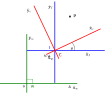
\includegraphics[width=\linewidth]{media/rot+trans-2D.pdf}
  \caption{The coordinate  frame $\{C\}$  is rotated around origin by an $\theta$
    from coordinate  frame $\{W\}$ and then shifted by translation ${}^w\bft_c$.}
  \label{fig:rot+trans-2D}
\end{figure}

\section{3D  Rotation matrix   from Euler  angles}
\section{3D  Transformation matrix}
\section{Axis-angle representation}
\section{Denavit-Hartenberg  transformations}
\section{Camera  projection model}
\section{Linear least squares  or  Pseudo-inverse}

\listoftheorems[ignoreall,show={defn}]

\end{document}